\section{Registration of AR Annotation on Social Video Sharing}
\label{sec:video}

AR annotation is an example of the interaction dimension on the Social AR Continuum. The registration of these annotations with respect to the user (viewer or sharer) can be represented in different level of detail (e.g., world-stabilised, body-stabilised and head-stabilised \cite{Billinghurst1998}) which can be mapped based on the social proximity. 

This section investigates an AR interface displaying comments directly on a live-streamed video. Our prototype allows remote spectators to perceive the streamed live video with different interfaces for displaying the comments, including an interface which puts AR annotation feedback directly on the shared video, and another interface that provides feedback in a separate window \cite{Nassani2016}. A user study was conducted to compare different ways of visualising comments and found that users prefer having comments directly in the AR view rather than in a separate list. This section discusses the implications of this research and directions for future work.

% Tobias: You did not really justify why you choose this specific visualisations/interfaces. You could state that it was inspired by YouTube or other media, but again, I think you need to justify your choice. Have there been other options, and why did you not choose them.

%  Tobias: You come directly from what the chapters do to your prototype. I would more appreciate if you integrate Figure 6.2 and use it to explain your envisioned scenario and context. From there, you can start to transition into the description of the prototype.

The vision of this work is to explore different user interfaces where users can add comments on a shared social video. Options considered based on existing video sharing platforms (e.g., YouTube\footnote{https://www.youtube.com/}, Vimeo\footnote{https://vimeo.com/}): (1) List, (2) Augmented Reality (AR), and (3) List + AR (see Figure \ref{fig:mgia16:conditions}).

\begin{figure}
  \includegraphics[width=\columnwidth]{images/61-video-mgia16/screenshots-enhanced-02}
  \caption{Overview of the investigated interfaces showing screenshots of the different interface conditions. (L): Comments displayed as a List on the side. (AR): Comments overlaid on the background video. (L+AR): Comments displayed both as a list on the right and as an overlay. }
  \label{fig:mgia16:conditions}
\end{figure}

Previous work has demonstrated live video sharing on a mobile platform and support for viewer feedback. However, there has been little evaluation of different methods for providing feedback. This section reports on investigations into different user interface (UI) options for viewing comments left by multiple users on a shared live video stream. Thus, the main contribution is investigating if comment placement on live video sharing improves the user experience. This work describes the prototype developed to explore this question.

\subsection{System Design}

In order to explore different ways to share AR comments from remote collaborators, a prototype was developed that enables a user to share a live video stream with others and receive comments from multiple users who are watching. Our system consists of a WebRTC\footnote{https://webrtc.org} application running on AppEngine\footnote{https://appengine.google.com/} on Google Cloud servers, which offers a fast peer-to-peer connection between devices. The advantage of the system being built on a web platform is that it can run on multiple hardware specifications, including desktop, hand-held, and wearable devices. Figure \ref{fig:mgia16:system} shows the overall design of the prototype system.

\begin{figure}[ht]
  \centering
  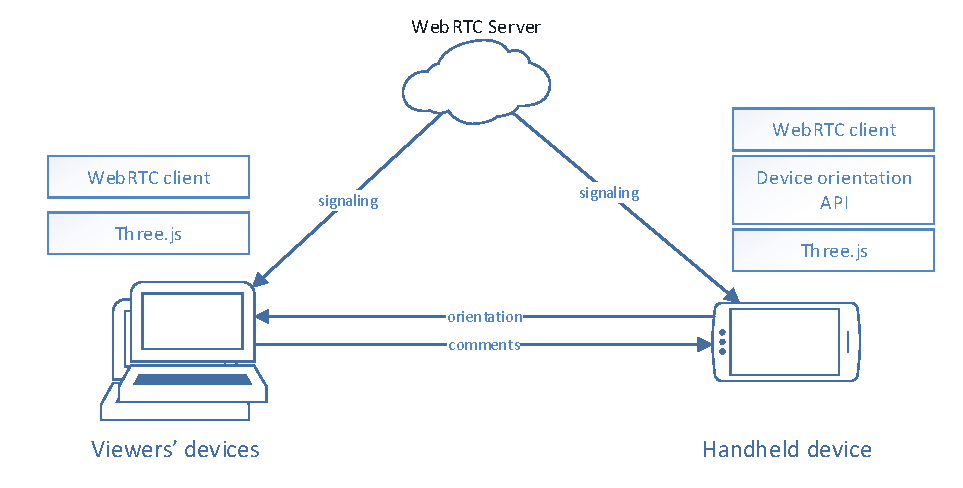
\includegraphics[width=\linewidth]{images/61-video-mgia16/system}
  \caption{System architecture of AR annotation on video streaming based on WebRTC}
    \label{fig:mgia16:system}
\end{figure}

The prototype was built as a fork from AppRTC\footnote{https://apprtc.appspot.com/} code base which hosts a website that enables people to start a video conferencing session on the web. The solution was built using an AppRTC base code was utilised to track device orientation by listening to the device sensors, and transferring the data to the receivers' devices via DataChannel. The AppRTC application is written in Python for the backend and Javascript for the front-end. It takes advantage of being hosted on AppSpot so that it complies with the WebRTC requirements for HTTPS. The AppRTC system allows users to communicate with each other over the Internet. The Three.js library\footnote{http://threejs.org/} was used. The AR visualization is implemented with two graphical layers (see Figure \ref{fig:mgia16:layers}). The background layer shows the video stream captured by the camera on the mobile device. On top of the background, comments are drawn on the front layer using orientation tracking information to show them in a body-stabilised manner. 

\begin{figure}[h]
  \centering
  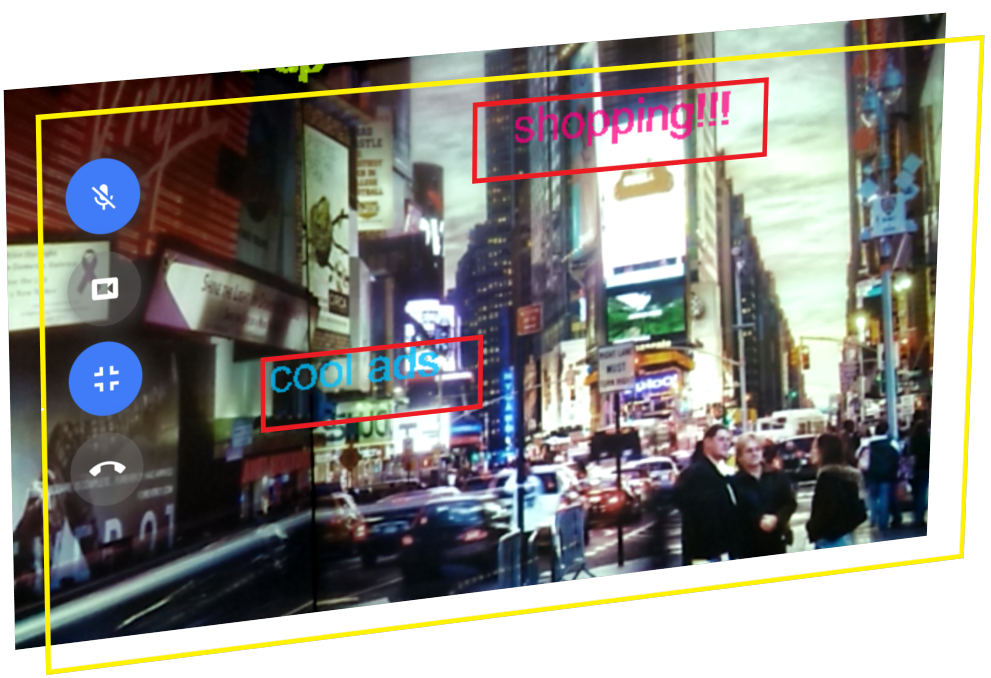
\includegraphics[width=0.8\linewidth]{images/61-video-mgia16/layers.png}
  \caption{UI of the system showing: 1) video layer (yellow) and 2) annotation layer (red)}
    \label{fig:mgia16:layers}
\end{figure}

\subsection{Implementation}

The application starts by turning on the back camera on the mobile device and asking the user to enter a "room number" to start the connection. Once this is entered, the application will enter "call mode", waiting for other participants to enter the same room number. Once the call is established, the mobile device will start streaming video and device orientation data to the viewing PC. 

Both users can send comments to each other by clicking on any part of the shared video. The system then calculates the 3D position of the comment in the AR space and waits for the comment text to be entered. Once the user enters the message, the text is displayed on both the sender's and receiver's screens. The motion data of the sender's device is also shared so that the receiver will see the comment appearing at the same place as the sender turns their device. 

Three different ways of showing comments on the live video stream are implemented (see Figure \ref{fig:mgia16:conditions} above). The first is a list view where the comments are listed on the side of the camera feed view. An AR view overlays comments on top of the video feed and rotated around the user based on phone orientation, so the comments appear fixed at the location on the video where they were first entered. Finally, an AR + list implementation combined the list view with the AR view. The next section reports on a user study exploring these three implementations.


\subsection{User Study}

A controlled within-subjects user experiment was conducted to test the different UIs for displaying comments, using the three approaches just explained. The experiment was approved by the Human Ethics Committee (HEC) and started with the participants giving consent and answering questions about demographic information. Then they went through a training session to get familiar with the application and the experimental procedures. The tasks during the training were designed to try to look around and read the comments appearing on the UI. A 180-degree panoramic image projected around the user on large screens was used to simulate different real spaces for the user (see Figure \ref{fig:mgia16:participant}). 

\begin{figure}[h]
  \centering
  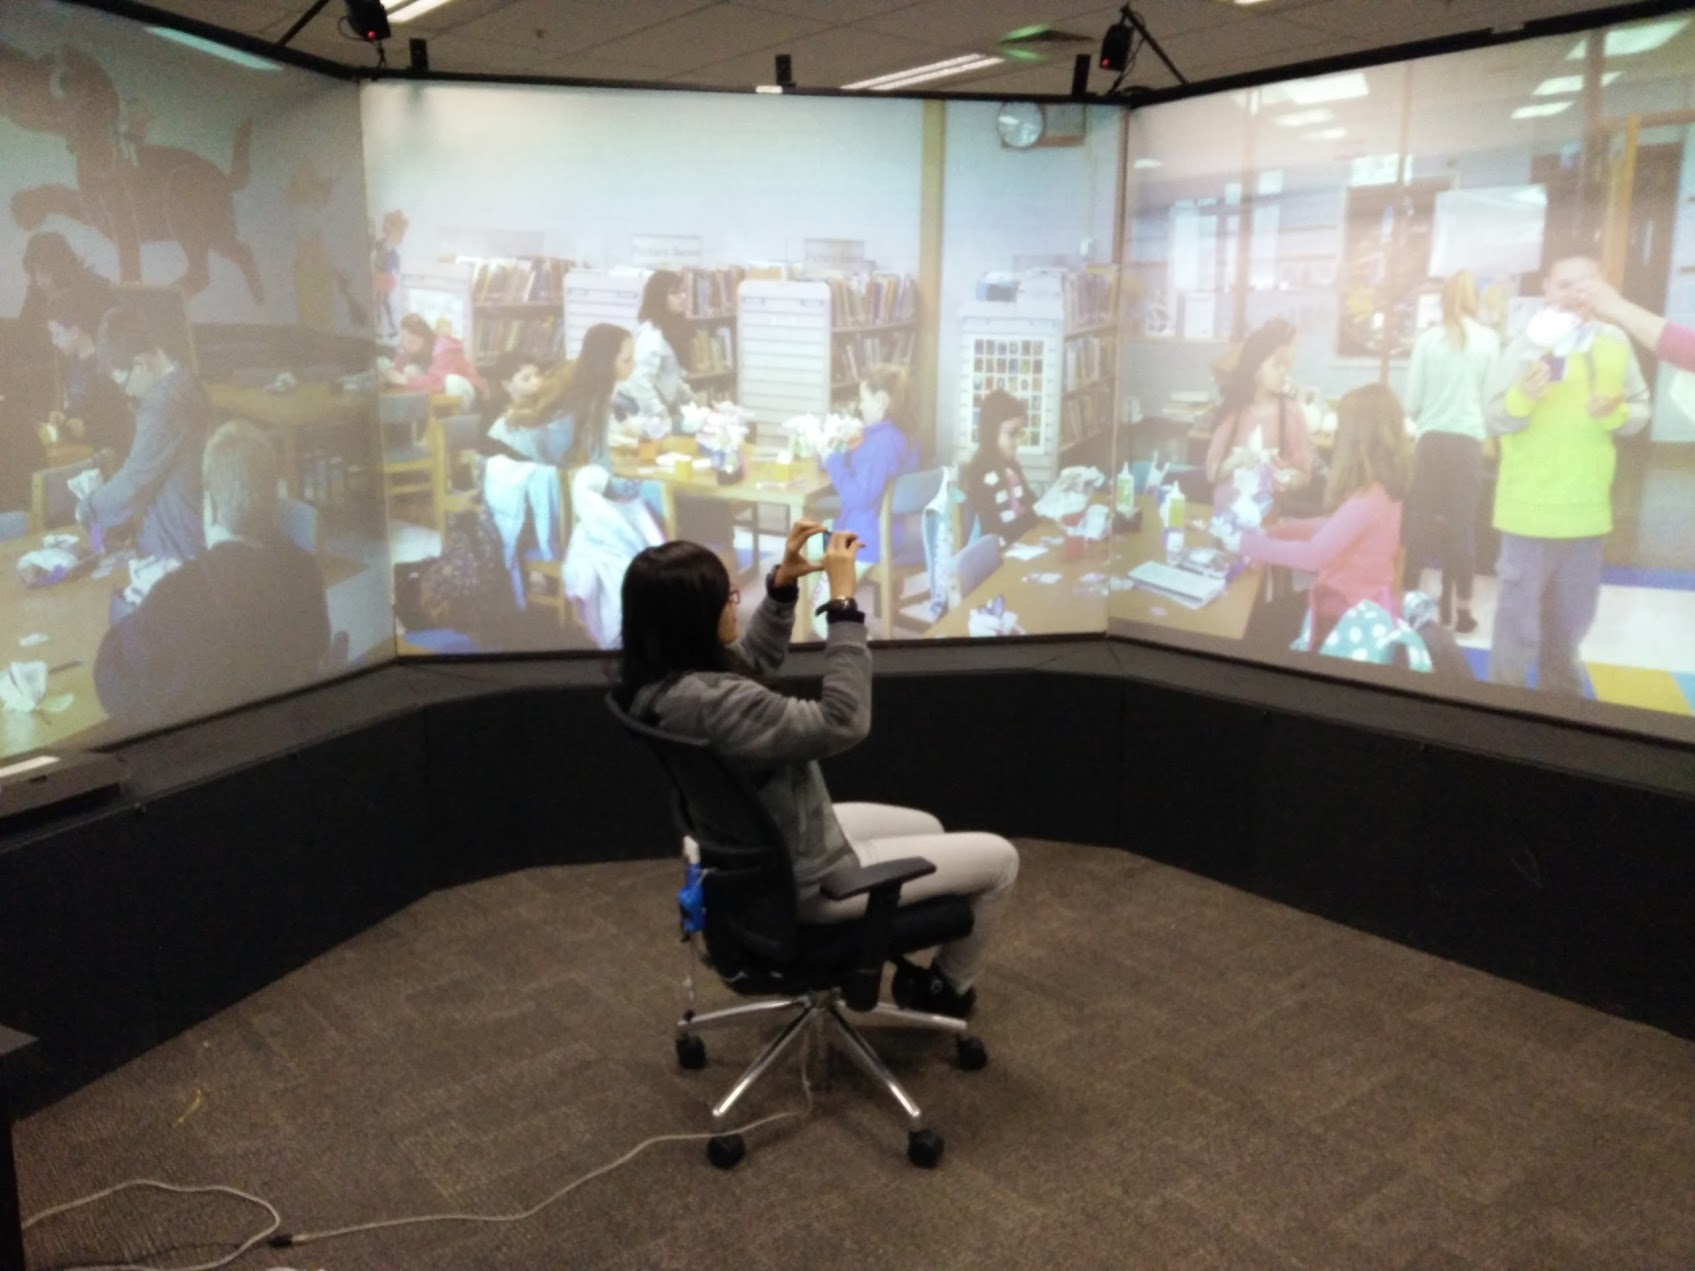
\includegraphics[width=0.45\linewidth]{images/61-video-mgia16/participant1}
  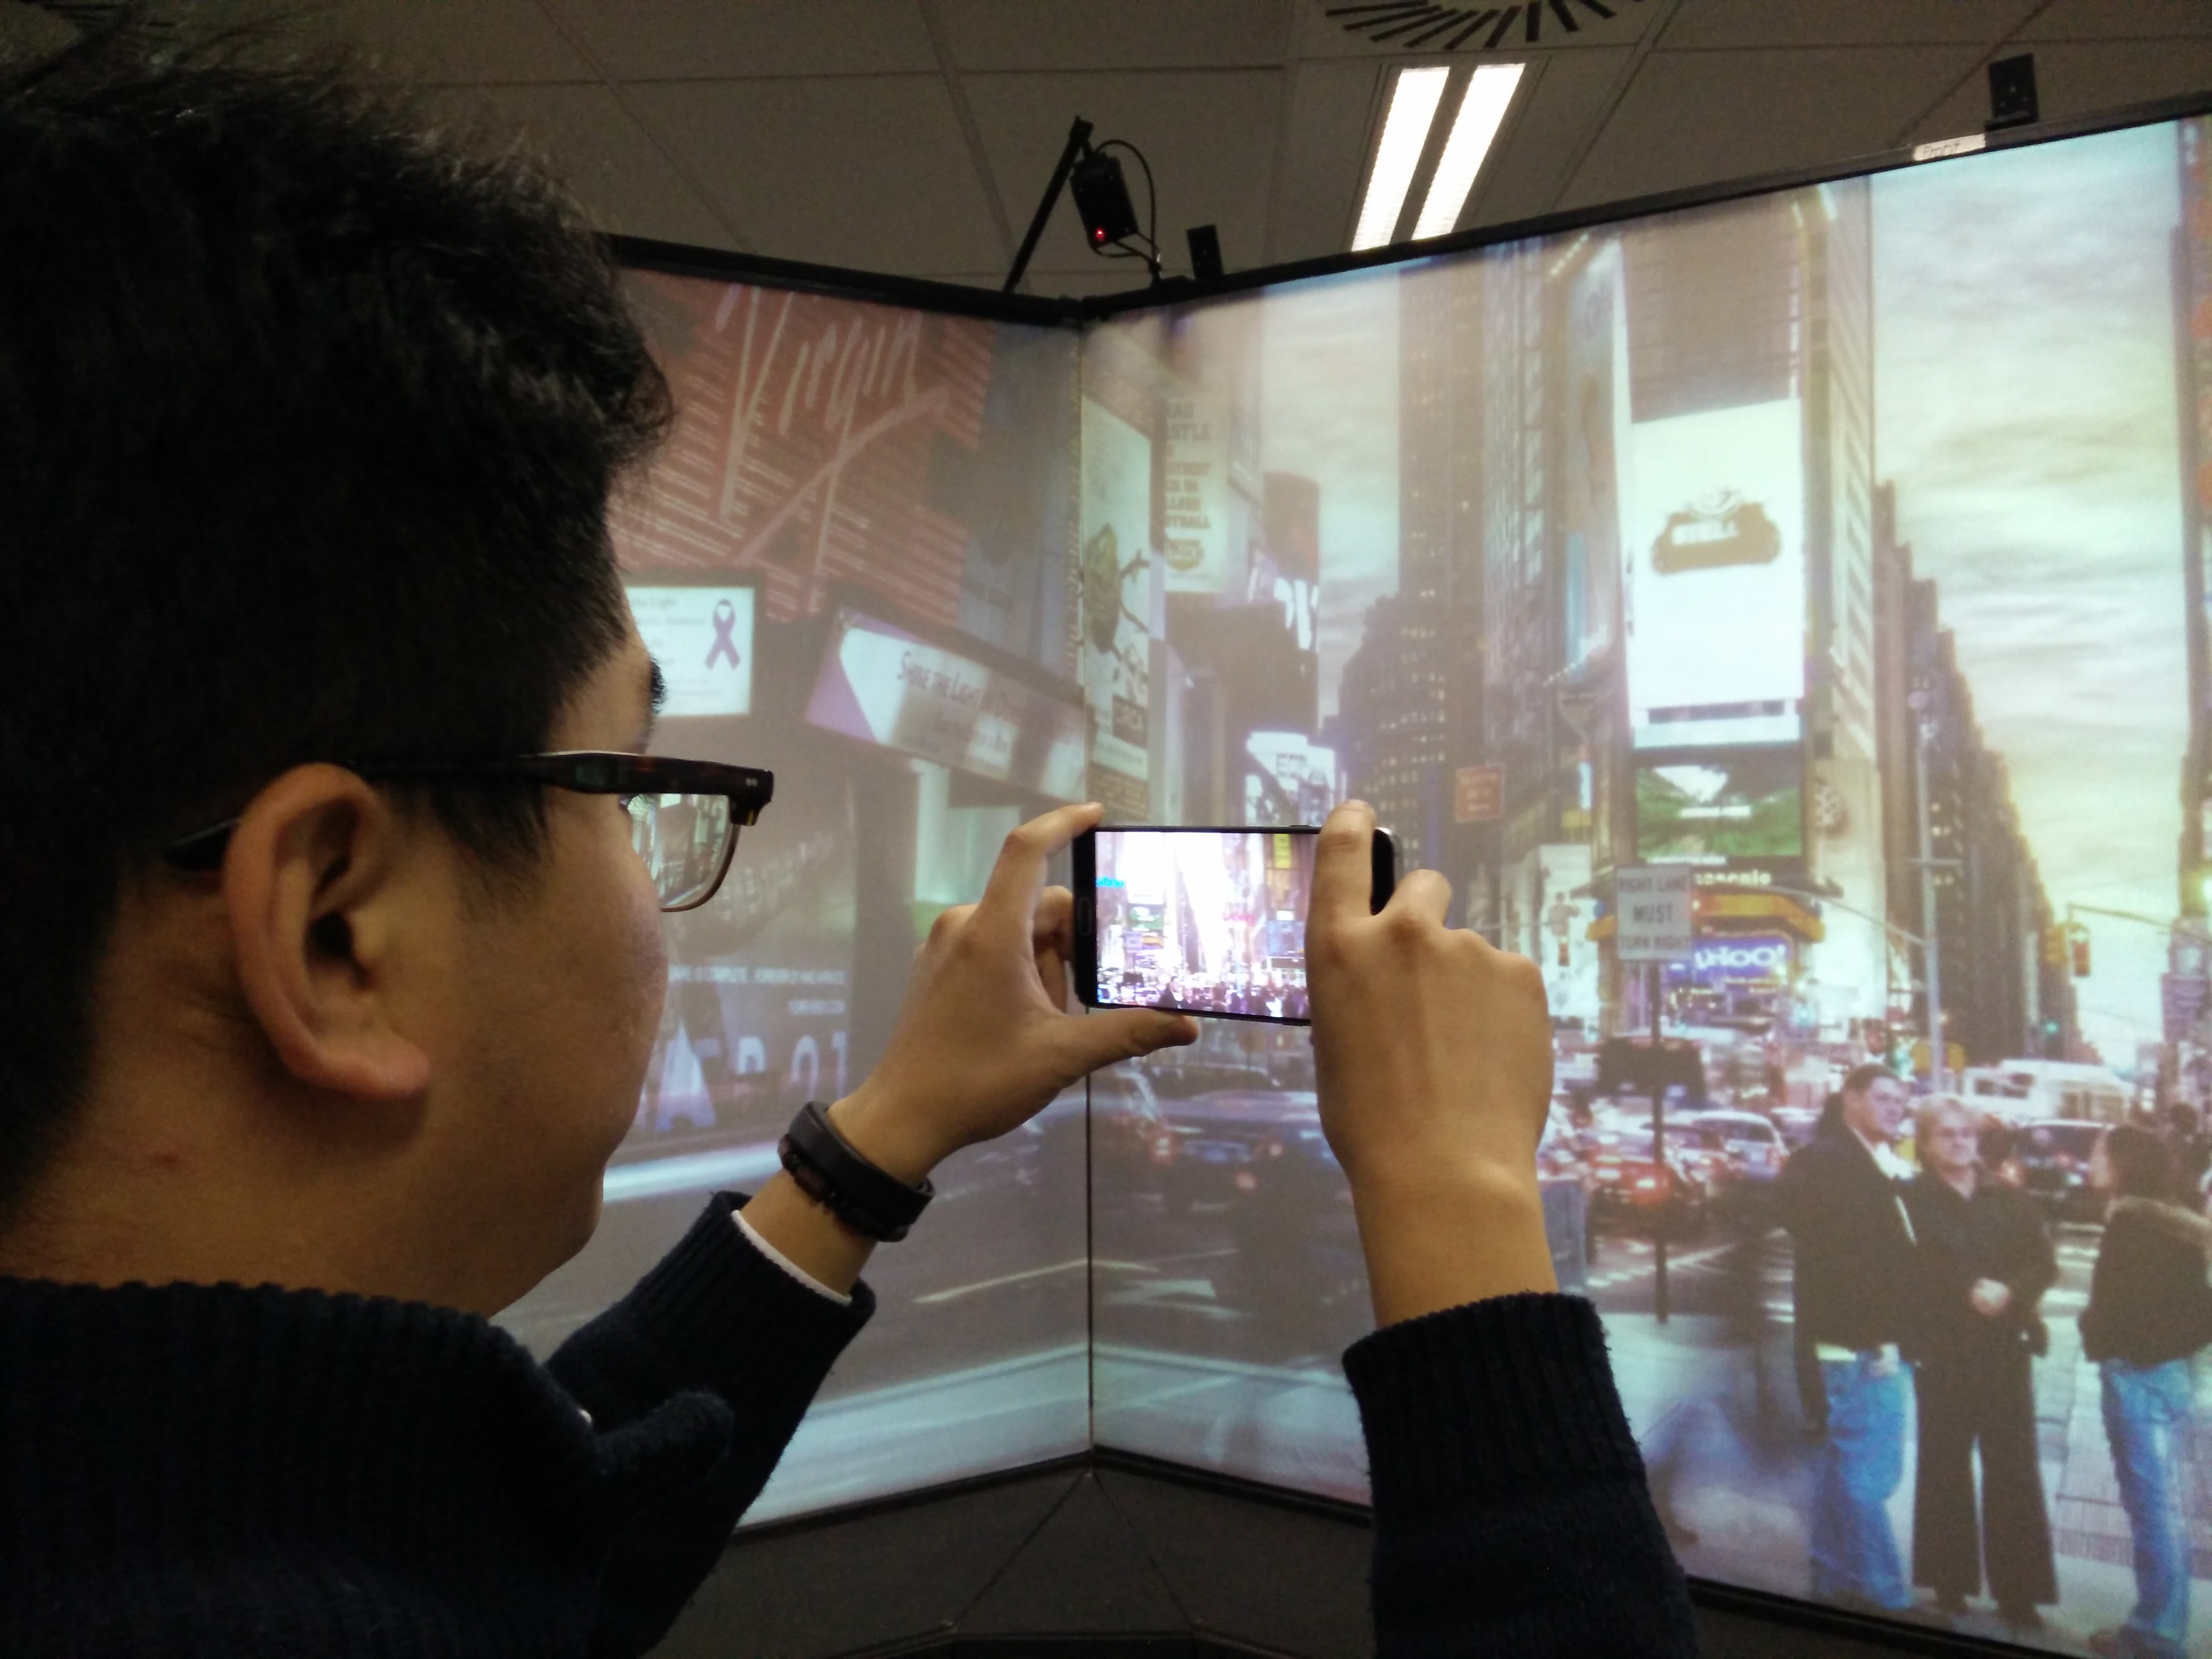
\includegraphics[width=0.45\linewidth]{images/61-video-mgia16/participant2}
  \caption{Participants during the experiment}
    \label{fig:mgia16:participant}
\end{figure}

Four different images were selected where the user might be interested in sharing their surroundings, varying in terms of indoors/outdoors and busy/quietness (see Figure \ref{fig:mgia16:backgrounds}). A different background was randomly assigned for each condition between subjects. 

\begin{figure}[h]
  \centering
  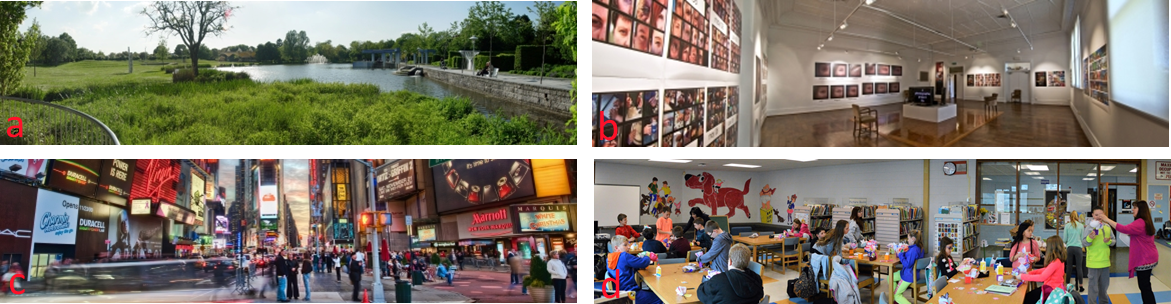
\includegraphics[width=\linewidth]{images/61-video-mgia16/backgrounds-legend.png}
  \caption{180-degree images used during the experiment. a) A park: outdoors and quiet, b) A museum: indoors and quiet, c) Intersection: outdoors and busy, d) A classroom: outdoors and busy.}
    \label{fig:mgia16:backgrounds}
\end{figure}

Each participant was asked to sit in the middle of the projection screens showing the background image, hold a smartphone, and aim its camera at the background to share it with remote users. The experimenter simulated multiple users sending comments on the shared video in a 'Wizard of Oz' style setup. There were six predefined comments (see Table \ref{table:mgia16:comment}) for each background. The predefined comments allowed for a controlled experiment (i.e., the same text at the same location) and reduced the need to have participants playing the role of the commenter. 

The comments appeared on the screen in three different styles depending on the experimental condition. The order of the conditions was counterbalanced using a balanced Latin square design. While watching the comments, the participant was asked to remember which part of the background each comment was talking about and who made a comment, which could be identified by the colour of the comment. There were up to four colours (commenters) in the experiment. The comments faded away one minute after being displayed, simulating the user receiving multiple comments while having limited time to read them all.

\begin{table}[h]
  \centering
  \caption{Social comments appeared on the 360 panoramic images during experiments}
  \label{table:mgia16:comment}
  \begin{tabular}{ |c|c|c|c| } 
\hline
    B1: Park    & B2: Museum  &   B3: Intersection    &  B4: Classroom\\
\hline
    nice place  &   interesting &  too many people & interesting \\
    picnic area &   beautiful   &  exciting  & busy \\
    play area   &   weird   &  shopping!!! & teacher \\
    nice lake   &   how much?    &  cool ads    & boring \\
    relaxing    &   confusing   &  people    & alone \\
    good for running    &   nice composition    &  traffic jam & what time is it\\\hline
  \end{tabular}
\end{table}

After completing a condition, participants were asked to place a printed version of each comment on a background image, at the correct location, and with the correct colour, testing their knowledge of where each comment appeared. The participants were also requested to answer a questionnaire on system usability \cite{brooke1996sus} and social presence \cite{Harms2004}. The social presence questions were slightly modified to fit the scenario being tested and only focused on one-way communication. Table \ref{table:social_questions} shows the social presence questions that were answered on a seven-level Likert-like scale rating (1: strongly disagree - 7: strongly agree). 

\begin{table}[h]
  \centering
  \caption{Social presence questionnaire. Negative questions marked with (-)}
  \label{table:social_questions}
  \begin{tabular}{ll}
    Q1 & Comments from others were clear to me.          \\
    Q2 & It was easy to understand comments from others. \\
    Q3 (-) & Understanding others' comments was difficult.  \\
    Q4 & I could tell how others felt by my video sharing.\\
    Q5 (-) & Others' emotions were not clear to me.\\
    Q6 & I could describe others' feelings accurately.
  \end{tabular}
\end{table}

% [do you want to show system usability questions as well?]

After finishing all three conditions, participants answered a post-experiment questionnaire that asked them to rank and compare all three conditions in terms of strengths and weaknesses. Finally, the experiment ended with a debriefing and the opportunity for participants to provide open-ended comments.

\subsection{Results}

Twenty participants (11 female, aged between 19 and 35 years old, Median=27.5, SD=4.55) were recruited to participate in the user study. Most (95\%) of them had experience with live video streaming a few times a week to a few times per month, and 80\% were familiar with AR applications. A Shapiro-Wilk test indicated that the data was not normally distributed. A non-parametric Friedman test was run for all the results with alpha=0.05, and post-hoc tests using Wilcoxon signed-rank tests with the Bonferroni correction ($alpha=0.017$).

The average SUS scores for each condition are shown in Figure \ref{fig:mgia16:questions_sus}. There was a statistically significant difference between the average SUS scores for each condition ($\chi^2(2)=9.658, p=0.008$). Post-hoc analysis showed significant differences between L and AR ($Z=-2.638, p=0.008$) and between L and L+AR ($Z=-2.559, p=0.010$). However, there was no statistically significant difference between AR and L+AR ($Z=-0.197, p=0.844$). This shows that the list condition on its own was considered considerably less usable than the other two conditions.

\begin{figure}[htb]
  \centering
  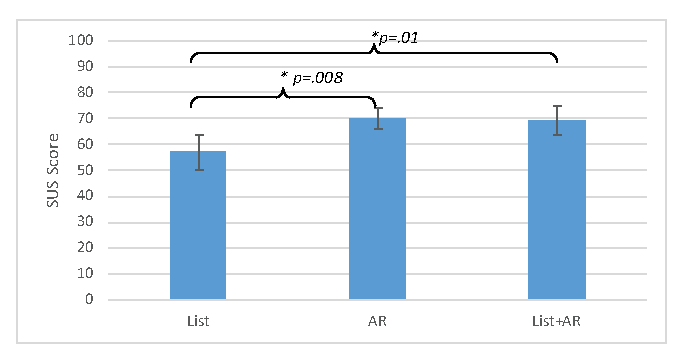
\includegraphics[width=0.8\linewidth]{images/61-video-mgia16/sus2.eps}
  \caption{SUS scores for each condition}
  \label{fig:mgia16:questions_sus}
\end{figure}

As for the social presence questions (see Figure \ref{fig:mgia16:social_presence}), the responses were inverted on the negative questions, Q3 and Q5, to allow all questions to be aggregated, combining the answers for both `perceived message understanding' and `perceived affective understanding' sub-scales. There was a statistically significant difference in the perceived social presence ($\chi^2(2)=16.892, p<0.001$). Post-hoc analysis found there were significant differences between L and AR ($Z=-3.459, p=0.001$) and between L and L+AR ($Z=-3.311, p=0.001$) while there was no statistically significant difference between AR and L+AR ($Z=-0.427, p=0.670$). 

% This shows that the list condition (L) was perceived as being less mutual understand and therefore creating less social presence, and that viewer comments in this condition were less clear.

% Why do you think there was a difference between AR and L+AR for the comment placement accuracy? It would be good to discuss this.

\begin{figure}[htb]
  \centering
  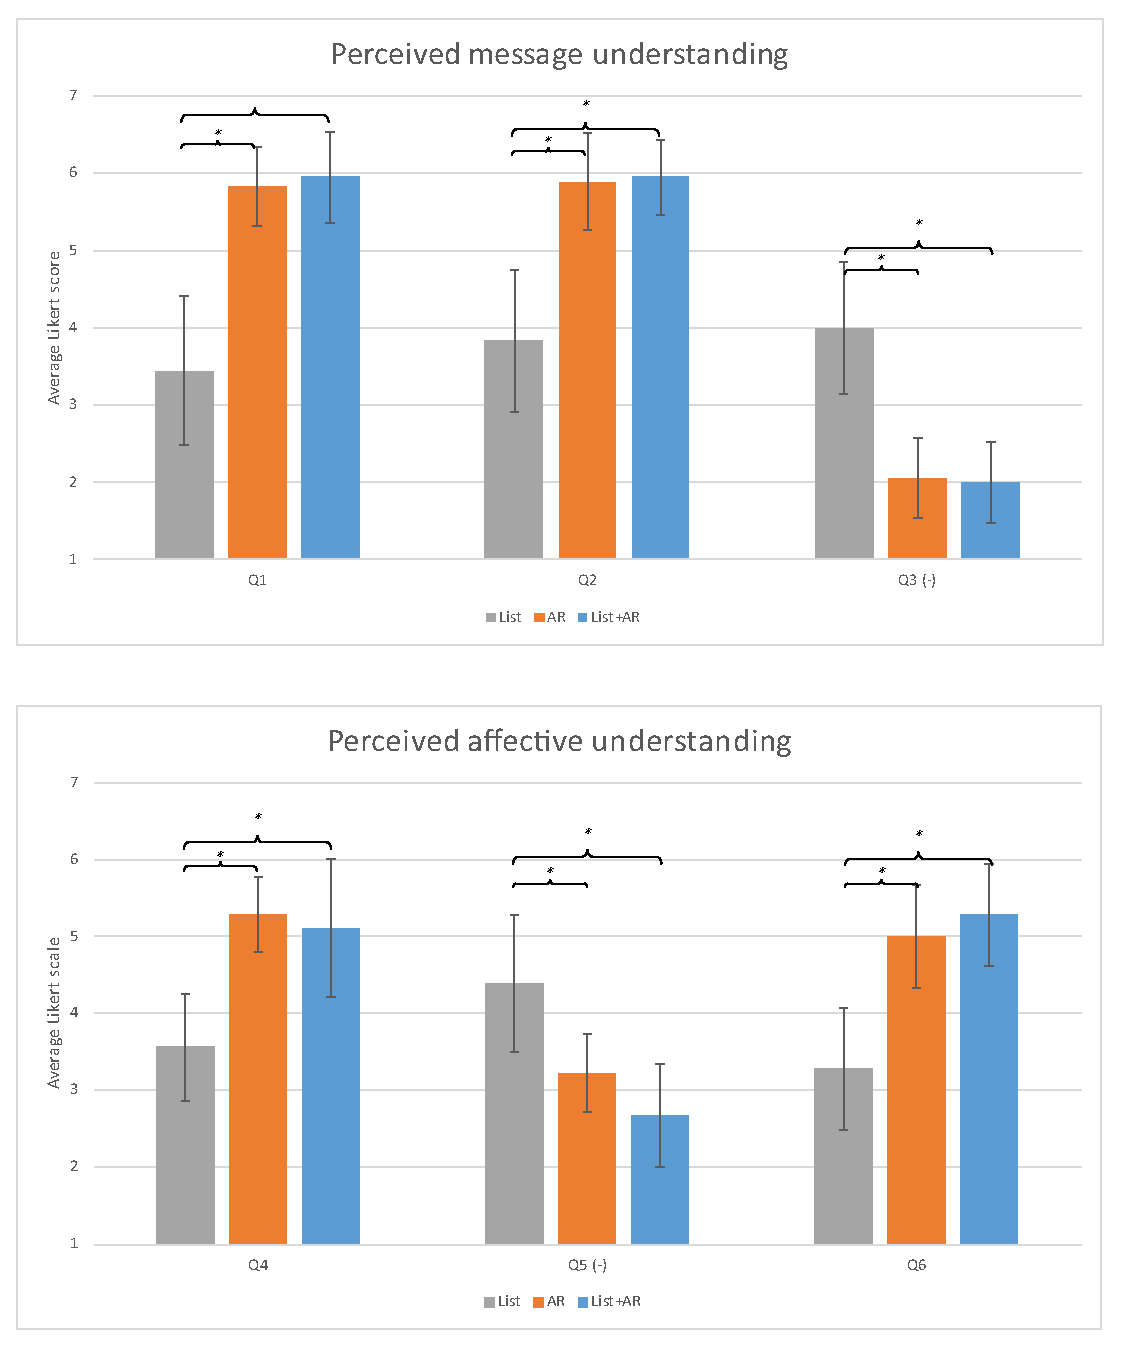
\includegraphics[width=\linewidth]{images/61-video-mgia16/social-presence.eps}
  \caption{Results for the social presence questions "perceived message understanding" and "perceived affective understanding". Whiskers indicate standard error. *=statistically significant difference}
    \label{fig:mgia16:social_presence}
\end{figure}

As for the ranking results (see Figure \ref{fig:mgia16:ranking}), the average of the answers (where 3=best, 1=worst) was calculated. The results show a statistically significant difference between conditions ($\chi^2(2)=9.100, p=0.011$). Post-hoc analysis showed a significance level set at $alpha$=0.017. There were significant differences between L and AR ($Z=-2.766, p=0.006$) and between L and L+AR ($Z=-2.502, p=0.012$). However, there was no statistically significant difference between AR and L+AR ($Z=-0.039, p=0.969$). This shows that the list condition (L) was ranked the worst out of the three conditions, and the two AR conditions were ranked the same.

\begin{figure}[htb]
  \centering
  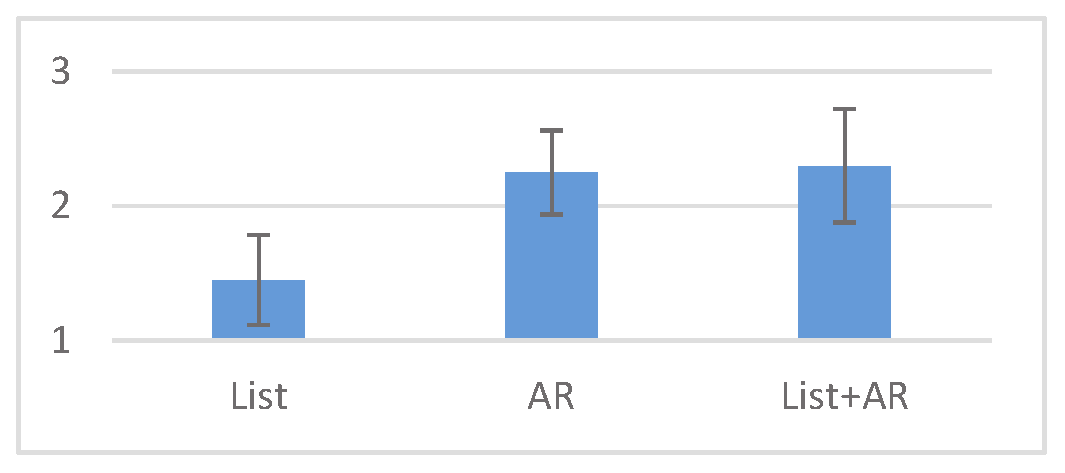
\includegraphics[width=.8\linewidth]{images/61-video-mgia16/ranking.eps}
  \caption{Results for condition ranking questions (3=best, 1=worst). Whiskers indicate standard error.}
    \label{fig:mgia16:ranking}
\end{figure}

For the task of matching the position and colour of the comments (see Figure \ref{fig:mgia16:questions_matching}) participants were asked to remember who wrote which comment (indicated by the colour of the comment) and the position of the comment (indicating which part of the scene the comment was about). The results show that there was a statistically significant difference ($\chi^2(2)=22.030, p<0.001$). Post-hoc analysis showed that there was no significant difference between the AR and L+AR conditions ($Z=-1.016, p=0.310$). However, there was a statistically significant difference between L and L+AR ($Z=-3.628, p<0.001$) and between L and AR conditions ($Z=-3.447, p=0.001$).

\begin{figure}[thb]
  \centering
  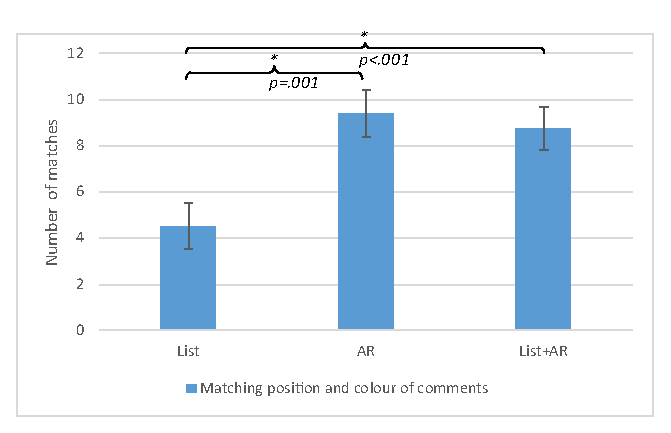
\includegraphics[width=.8\linewidth]{images/61-video-mgia16/matching-02.eps}
  \caption{Results for correctly matching comments with background and colour. Whiskers indicate standard error. *=statistically significant difference.}
    \label{fig:mgia16:questions_matching}
\end{figure}

Participants were asked open-ended questions to comment on their experience in terms of the strengths and the weaknesses of each condition. Approximately 80\% of feedback from the participants noted that in the list condition (L) it was more difficult to identify the area of the comments compared to the AR conditions. Eight participants (40\%) found it more challenging to remember the comment colours as a means to identify the person who sent the comment. 

In the AR and L+AR conditions, participants felt that the comments were contextual and relevant to the background. For example, \textit{"It is easier to remember comments on the video (AR) because the comments act as cues on the video you can directly see what the people are commenting on which I think makes me feel more connected to them"}. One of the strengths of the L+AR condition commented on included having an overview of the list of comments even if they are outside the current viewpoint of the user. 

However, users felt that comments in the L+AR condition could clutter the UI and partially block the background. One participant said \textit{"The screen just became too busy with comments that I do not have the time to actually sort out the comments and associate them on the video"}. Some suggested this could be resolved by making the comments not in the centre of view more transparent.
 
Participants were asked what they would like to improve. Most reported that they would like to use a head-mounted display to view comments in the AR mode.  It was also suggested to use a profile image instead of colours on comments to distinguish remote users.
 
Overall users felt that the AR and L+AR conditions were fun and cool to use, providing comments such as \textit{"It is pretty awesome. I love the experience, and I would really like to use this app with my social network."}.


\subsection{Discussion}

The user study results found that subjects preferred the conditions that contained an AR view, compared to showing comments only displayed in a list format. They thought these AR conditions were more usable than non-AR, provided a higher degree of social presence, and enabled them to remember the comment layout better. This is probably because the spatial association of comments increases the likelihood of the message being understood.
% Why do you think there was a difference between AR and L+AR for the comment placement accuracy? It would be good to discuss this

It was expected that one of the AR conditions (AR or L+AR) would have been more popular than the other; however, this was not the case. Some users preferred L+AR over the AR as the former provided an overall list of comments even if they were not visible in the current user viewpoint, making the user more aware of new comments without needing to look around to find them. Other users preferred the AR only condition, as the screen was less crowded. One solution to this might be hiding the comments on the list that are visible on the AR view, removing any duplication. Alternatively, a radar view could be used to show dots to represent comments. 

% It was learned that more about how to make live streaming a better experience for the user. 
Some users found the one-minute timeout for the comments fading away to be too fast. Associating the comments with colour to represent different users may not be the best option. An alternative approach would be to use an avatar or name of the person to identify the comment source. 

The study has a number of limitations that have to be addressed in the future. The experiment was conducted in a simulated environment rather than outdoors. A static background image was used to simplify the conditions. However, in real life, things will be moving in the background (e.g., people walking, cars passing by). In such scenarios, the comments in the AR condition may not stick to the moving objects. However, this could be solved by using image processing techniques to track objects that will allow the comment to be moved with them. Finally, all of the comments were generated by an experimenter and were fixed, rather than coming from real people who could write whatever they liked.    

\subsection{Conclusions}

This section investigated AR annotations for social live video streaming. The work included conducting a user study testing three variations of the interface for showing comments: 1) a List view, 2) an AR view and 3) a combined List + AR view. Participants felt that the AR and the List + AR conditions were significantly better than the List condition in terms of system usability and social presence. The following sections investigate the higher level of fidelity in AR annotations using 3D sensors and on panoramic images. 